
In order to validate a 


\graphicspath{{img/results/}}

\begin{figure*}
    \centering
    \begin{subfigure}[t]{0.3\textwidth}
        % \centering
        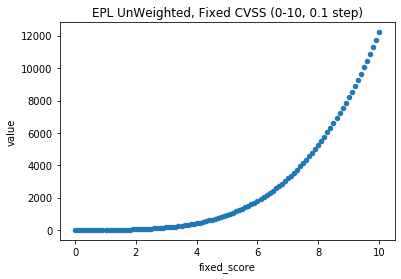
\includegraphics[width=\linewidth]{output_37_1.png} 
        \caption{Distribution of observed non-normalized EPL} 
        \label{fig:refnet_small}
    \end{subfigure}
          \begin{subfigure}[t]{0.3\textwidth}
        \centering
        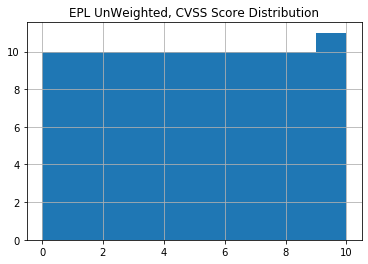
\includegraphics[width=\linewidth]{output_37_2.png}
        \caption{CVSS fixed uniformly}
        \label{fig:refnet_med}
    \end{subfigure}
     \begin{subfigure}[t]{0.3\textwidth}
        \centering
        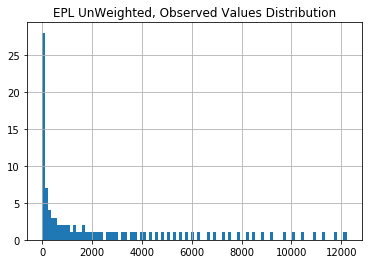
\includegraphics[width=\linewidth]{output_37_3.png}
        \caption{Exponential Distribution of EPL scores without normalization}
        \label{fig:refnet_large}
    \end{subfigure}
    \hfill
    \caption{Non-Normalized CVSS-weighted EPL (0-10, 0.1steps)}
    \label{fig:unweighted_epl}
\end{figure*}

\begin{figure*}
    \centering
    \begin{subfigure}[t]{0.3\textwidth}
        % \centering
        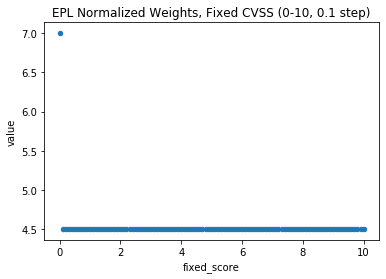
\includegraphics[width=\linewidth]{output_31_1.png} 
        \caption{Normalizing counters the effect of CVSS scoring} 
        \label{fig:norm_epl}
    \end{subfigure}
          \begin{subfigure}[t]{0.3\textwidth}
        \centering
        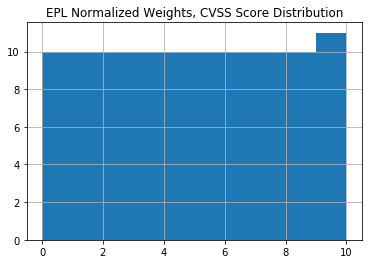
\includegraphics[width=\linewidth]{output_31_2.png}
        \caption{CVSS fixed uniformly}
        \label{fig:refnet_med}
    \end{subfigure}
     \begin{subfigure}[t]{0.3\textwidth}
        \centering
        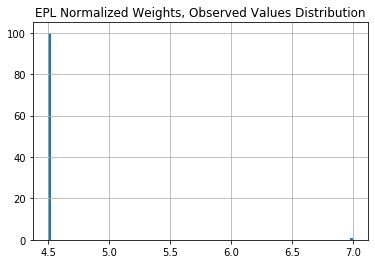
\includegraphics[width=\linewidth]{output_31_3.png}
        \caption{All observed values nearly identical}
        \label{fig:refnet_large}
    \end{subfigure}
    \hfill
    \caption{Average timings (in seconds) for 100 non-normalized EPL tests }
    \label{fig:weighted_epl}
\end{figure*}

\begin{figure}
    \centering
    \begin{subfigure}[t]{0.3\textwidth}
        % \centering
        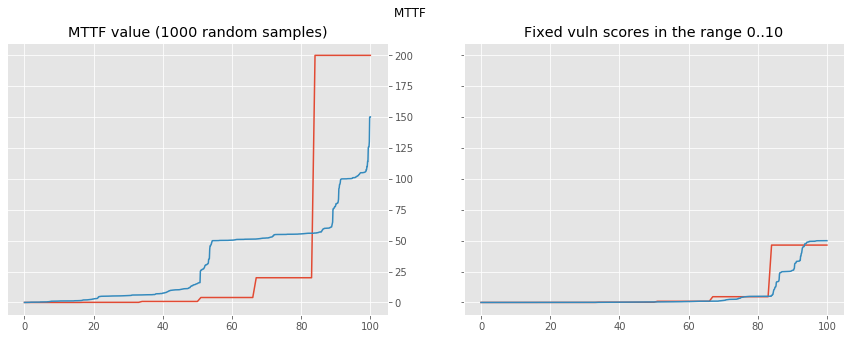
\includegraphics[width=\linewidth]{output_44_0.png} 
        \caption{Normalizing counters the effect of CVSS scoring} 
        \label{fig:norm_epl}
    \end{subfigure}
          \begin{subfigure}[t]{0.3\textwidth}
        \centering
        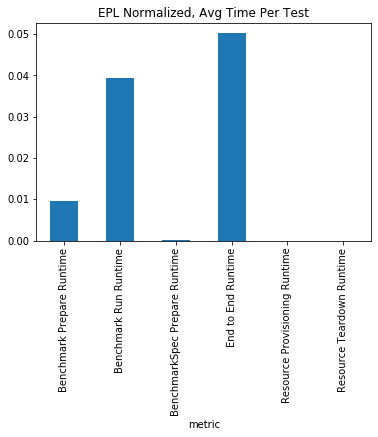
\includegraphics[width=\linewidth]{output_47_0.png}
        \caption{Average timings (in seconds) for 100 normalized EPL tests }
        \label{fig:norm_timings}
    \end{subfigure}
        \hfill
    \caption{Mean times in each stage of the evaluation pipeline}\label{fig:timings}
\end{figure}

% \begin{figure}
%     \centering
%     \begin{subfigure}[t]{1in}        
%         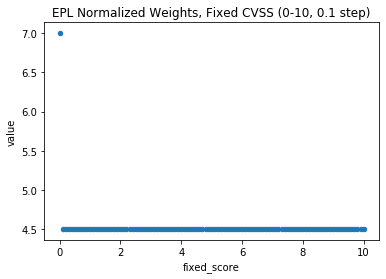
\includegraphics[width=1in]{output_31_1.png}     
%         \caption{}
%     \end{subfigure}    
    
%     \begin{subfigure}[t]{1in}        
%         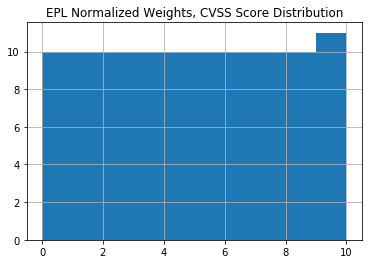
\includegraphics[width=1in]{output_31_2.png}  
%         \caption{}
%     \end{subfigure}
    
%     \medskip  % <-------------------------------  
    
%     \begin{subfigure}[t]{1.5in}
%         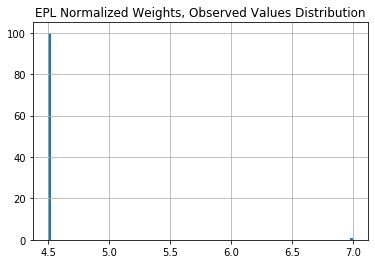
\includegraphics[width=1.5in]{output_31_3.png}
%         \caption{}
%     \end{subfigure}    
     
%      \begin{subfigure}[t]{1.5in}            
%         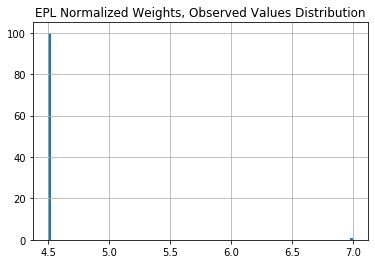
\includegraphics[width=1.5in]{output_31_3.png}   
%         \caption{}
%     \end{subfigure}
    
%     \medskip  % <------------------------------- 
    
%     \begin{subfigure}[t]{1.5in}
%         \centering
%         % \caption{Prelec}
%             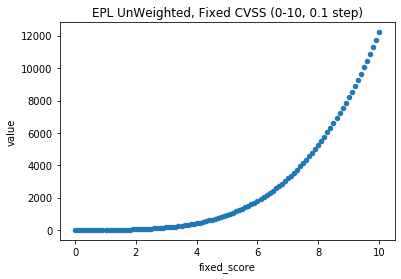
\includegraphics[width=1.5in]{output_37_1.png}  
%             \caption{}
%     \end{subfigure}
    
% %            \caption{Prelec}%\label{fig:2b}
%     \begin{subfigure}[t]{1.5in}
%         \centering
%                 % \caption{Prelec}
%         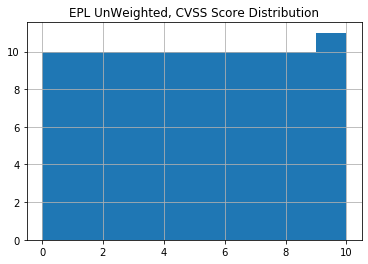
\includegraphics[width=1.5in]{output_37_2.png} 
%         \caption{}
%     \end{subfigure}
    
    
    
    
        
%     \centering
%     \caption{Classifier Error Plots (Predicted vs Actual) for the system's calculated security}\label{fig:ml:classifier_errors} 
% \end{figure}
